%!TeX root=../tese.tex
%("dica" para o editor de texto: este arquivo é parte de um documento maior)
% para saber mais: https://tex.stackexchange.com/q/78101/183146

%% ------------------------------------------------------------------------- %%
\chapter{Uma introdução à Teoria dos Grafos}
\label{cap:introducao}

\section{As Pontes de Königsberg}

No século XVIII, a cidade de Königsberg, na Prússia (hoje Kaliningrado, na  atual 
Rússia) era um importante centro comercial devido à sua localização próxima ao rio,
que dividia a cidade em quatro regiões, interligadas por sete pontes.

\begin{figure}
  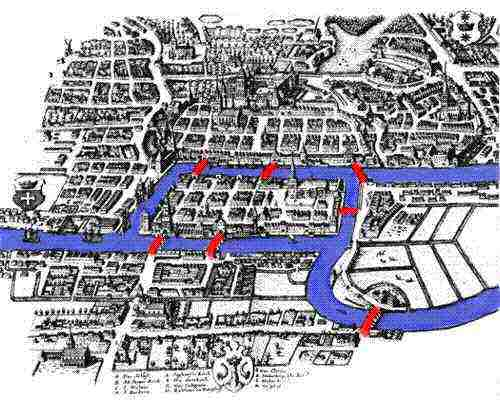
\includegraphics[scale=0.5]{Konigsberg.jpeg}
  \caption{A cidade de Königsberg e suas sete pontes}
\end{figure}

Segundo histórias, um passatempo de domingo dos cidadãos de Königsberg consistia em
passear por sua cidade, até que um dia surgiu um desafio: encontrar uma forma
de andar por todas as regiões passando por cada ponte apenas uma vez.

Nenhum habitante de Königsberg conseguiu encontrar a solução para este problema,
porém, o desafio chegou até um homem chamado Leonhard Euler, que apesar de julgar
o problema trivial, ficou intrigado, como citado em \citet{hopkins04:the}:

\begin{quotation}
  \emph{``This question is so banal, but seemed to me worthy of attention in that 
  [neither] geometry, nor algebra, nor even the art of counting was sufficient to
  solve it.''}
\end{quotation}

Euler provou que não era possível passar por toda a cidade de Königsberg sem passar
duas vezes pela mesma ponte, mas também resolveu o caso geral,
para qualquer número de regiões e qualquer número de pontes, dando assim origem
a um ramo da matemática que hoje chamamos de \textbf{Teoria dos Grafos}.

\section{Grafos}

Podemos definir um \textbf{Grafo} informalmente como um conjunto de entidades
conectadas entre si (ou não). Mais formalmente, podemos definir um grafo $G$ como um
par $(V, E)$ onde $V$ é um conjunto de \textbf{vértices} e $E$ um conjunto de
\textbf{arestas} entre os vértices tal que $E \subseteq \{ (u, v) \mid u, v \in V \}$.

As arestas de um grafo podem ter propriedades como direção e/ou algum valor
associado dependendo do contexto em que está sendo utilizado, frequentemente
possibilitando soluções elegantes e eficientes para os mais diversos problemas.

\begin{figure}
  \centering
  \subcaptionbox{Um grafo não dirigido.\label{fig:subfigures:a}}
    [0.45\textwidth]{
      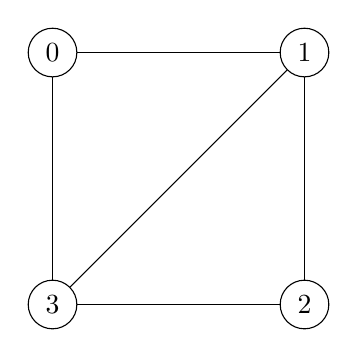
\begin{tikzpicture}[scale=.8]
        \tikzstyle{node_style} = [circle,draw=black]
        \tikzstyle{edge_style} = [draw=black]
        \node[node_style] (v1) at (-2,2) {0};
        \node[node_style] (v2) at (2,2) {1};
        \node[node_style] (v4) at (2,-2) {2};
        \node[node_style] (v5) at (-2,-2) {3};
        \draw[edge_style]  (v1) edge (v2);
        \draw[edge_style]  (v4) edge (v5);
        \draw[edge_style]  (v5) edge (v1);
        \draw[edge_style]  (v5) edge (v2);
        \draw[edge_style]  (v4) edge (v2);
      \end{tikzpicture}
  }
  \subcaptionbox{Um grafo dirigido.\label{fig:subfigures:b}}
    [0.45\textwidth]{
      \begin{tikzpicture}[scale=.8]
        \tikzstyle{node_style} = [circle,draw=black]
        \tikzstyle{edge_style} = [draw=black, ->,> = latex']
        \node[node_style] (v1) at (-2,2) {0};
        \node[node_style] (v2) at (2,2) {1};
        \node[node_style] (v4) at (2,-2) {2};
        \node[node_style] (v5) at (-2,-2) {3};
        \draw[edge_style]  (v1) edge (v2);
        \draw[edge_style]  (v4) edge (v5);
        \draw[edge_style]  (v5) edge (v1);
        \draw[edge_style]  (v5) edge (v2);
        \draw[edge_style]  (v4) edge (v2);
      \end{tikzpicture}
  }
  \\
  \vspace{1cm}
  \subcaptionbox{Um grafo com valores nas arestas.\label{fig:subfigures:c}}
    [0.45\textwidth]{
      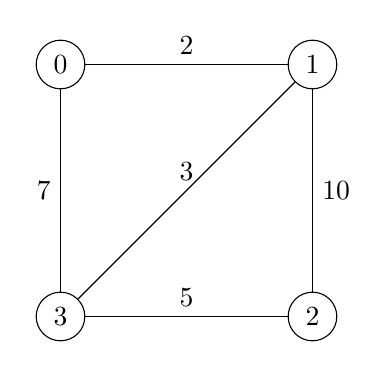
\begin{tikzpicture}[scale=.8]
        \tikzstyle{node_style} = [circle,draw=black]
        \tikzstyle{edge_style} = [draw=black]
        \node[node_style] (v1) at (-2,2) {0};
        \node[node_style] (v2) at (2,2) {1};
        \node[node_style] (v4) at (2,-2) {2};
        \node[node_style] (v5) at (-2,-2) {3};
        \draw[edge_style]  (v1) -- (v2) node[midway, above] {$2$};
        \draw[edge_style]  (v4) -- (v5) node[midway, above] {$5$};
        \draw[edge_style]  (v5) -- (v1) node[midway, left] {$7$};
        \draw[edge_style]  (v5) -- (v2) node[midway, above] {$3$};
        \draw[edge_style]  (v4) -- (v2) node[midway, right] {$10$};
      \end{tikzpicture}
  }
  \subcaptionbox{Um grafo dirigido com valores nas arestas.\label{fig:subfigures:d}}
    [0.45\textwidth]{
      \begin{tikzpicture}[scale=.8]
        \tikzstyle{node_style} = [circle,draw=black]
        \tikzstyle{edge_style} = [draw=black, ->,> = latex']
        \node[node_style] (v1) at (-2,2) {0};
        \node[node_style] (v2) at (2,2) {1};
        \node[node_style] (v4) at (2,-2) {2};
        \node[node_style] (v5) at (-2,-2) {3};
        \draw[edge_style]  (v1) -- (v2) node[midway, above] {$2$};
        \draw[edge_style]  (v4) -- (v5) node[midway, above] {$5$};
        \draw[edge_style]  (v5) -- (v1) node[midway, left] {$7$};
        \draw[edge_style]  (v5) -- (v2) node[midway, above] {$3$};
        \draw[edge_style]  (v4) -- (v2) node[midway, right] {$10$};
      \end{tikzpicture}
  }
  \caption{Exemplos de grafos.\label{fig:subfigures}}
\end{figure}

\section{Árvores}

\textbf{Árvores} são um subconjunto dos grafos de incrível importância para a
Ciência da Computação, sendo usadas nas mais diversas aplicações, desde a estrutura
de pastas de um sistema operacional até bancos de dados e processamento de
linguagem natural.

Diferente de outras estruturas como vetores, as árvores se organizam de forma
não linear, hierárquica. Os elementos de uma árvore são chamados de \textbf{nós} e
comumente um nó específico é elegido para ser a sua \textbf{raiz}. Cada nó pode
ter ligações com outros nós denominados \textbf{filhos}, que por sua vez podem
ter seus próprios filhos e assim sucessivamente até chegarmos em nós que não
possuem ligação com nenhum outro elemento; chamamos estes nós de \textbf{folhas}.
Também definimos a \textbf{profundidade} de um nó como a quantidade de arestas no
caminho da raiz até ele, ou seja, a raiz tem profundidade zero, seus filhos
profundidade um e assim sucessivamente. Cada \textbf{nível} da árvore corresponde a
uma ``fatia horizontal'' que contém os nós de uma certa profundidade; por definição, o
nível de um nó $u$ é \textit{profundidade(u) + 1}.

\begin{figure}
  \centering
  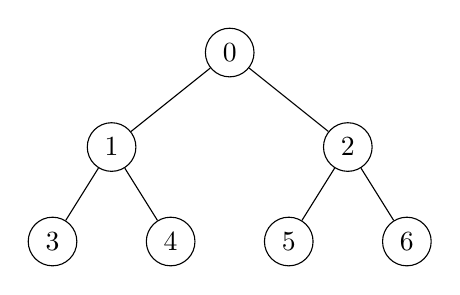
\begin{tikzpicture}[
    level distance=1.2cm,
    level 1/.style={sibling distance=3cm},
    level 2/.style={sibling distance=1.5cm}]
    \node [circle, draw] {0}
      child {node [circle, draw] {1}
        child {node [circle, draw] {3}}
        child {node [circle, draw] {4}}
      }
      child {node [circle, draw] {2}
        child {node [circle, draw] {5}}
        child {node [circle, draw] {6}
        % child [grow=right] {node (q) {$\qquad$} edge from parent[draw=none]
        %     child [grow=right] {node (q) {profundidade = 2, nível = 3} edge from parent[draw=none]
        %       child [grow=up] {node (r) {profundidade = 1, nível = 2} edge from parent[draw=none]
        %         child [grow=up] {node (s) {profundidade = 0, nível = 1} edge from parent[draw=none]
        %         }
        %       }
        %     }
        %   }
        }
      };
  \end{tikzpicture}
  \caption[Exemplo de árvore.]
  {\textbf{Exemplo de árvore.} O nó 0 é a raiz e tem como filhos os nós 1 e 2, cujos
  filhos são as folhas 3, 4 e 5, 6, respectivamente. O primeiro nível contém o nó 0 e
  tem profundidade zero, o segundo os nós 1 e 2 com profundidade um e o terceiro os nós
  3, 4, 5 e 6 com profundidade dois.}
  \end{figure}
  
  % \begin{tikzpicture}[level/.style={sibling distance=60mm/#1}]
    % \node [circle,draw] (z){$n$}
    %   child {node [circle,draw] (a) {$\frac{n}{2}$}
    %     child {node [circle,draw] (b) {$\frac{n}{2^2}$}
    %       child {node {$\vdots$}
    %         child {node [circle,draw] (d) {$\frac{n}{2^k}$}}
    %         child {node [circle,draw] (e) {$\frac{n}{2^k}$}}
    %       } 
    %       child {node {$\vdots$}}
    %     }
    %     child {node [circle,draw] (g) {$\frac{n}{2^2}$}
    %       child {node {$\vdots$}}
    %       child {node {$\vdots$}}
    %     }
    %   }
    %   child {node [circle,draw] (j) {$\frac{n}{2}$}
    %     child {node [circle,draw] (k) {$\frac{n}{2^2}$}
    %       child {node {$\vdots$}}
    %       child {node {$\vdots$}}
    %     }
    %   child {node [circle,draw] (l) {$\frac{n}{2^2}$}
    %     child {node {$\vdots$}}
    %     child {node (c){$\vdots$}
    %       child {node [circle,draw] (o) {$\frac{n}{2^k}$}}
    %       child {node [circle,draw] (p) {$\frac{n}{2^k}$}
    %         child [grow=right] {node (q) {$=$} edge from parent[draw=none]
    %           child [grow=right] {node (q) {$O_{k = \lg n}(n)$} edge from parent[draw=none]
    %             child [grow=up] {node (r) {$\vdots$} edge from parent[draw=none]
    %               child [grow=up] {node (s) {$O_2(n)$} edge from parent[draw=none]
    %                 child [grow=up] {node (t) {$O_1(n)$} edge from parent[draw=none]
    %                   child [grow=up] {node (u) {$O_0(n)$} edge from parent[draw=none]}
    %                 }
    %               }
    %             }
    %             child [grow=down] {node (v) {$O(n \cdot \lg n)$}edge from parent[draw=none]}
    %           }
    %         }
    %       }
    %     }
    %   }
    % };
    % \path (a) -- (j) node [midway] {+};
    % \path (b) -- (g) node [midway] {+};
    % \path (k) -- (l) node [midway] {+};
    % \path (k) -- (g) node [midway] {+};
    % \path (d) -- (e) node [midway] {+};
    % \path (o) -- (p) node [midway] {+};
    % \path (o) -- (e) node (x) [midway] {$\cdots$}
    %   child [grow=down] {
      %     node (y) {$O\left(\displaystyle\sum_{i = 0}^k 2^i \cdot \frac{n}{2^i}\right)$}
      %     edge from parent[draw=none]
      %   };
      % \path (q) -- (r) node [midway] {+};
      % \path (s) -- (r) node [midway] {+};
      % \path (s) -- (t) node [midway] {+};
      % \path (s) -- (l) node [midway] {=};
      % \path (t) -- (u) node [midway] {+};
      % \path (z) -- (u) node [midway] {=};
      % \path (j) -- (t) node [midway] {=};
      % \path (y) -- (x) node [midway] {$\Downarrow$};
      % \path (v) -- (y)
      %   node (w) [midway] {$O\left(\displaystyle\sum_{i = 0}^k n\right) = O(k \cdot n)$};
      % \path (q) -- (v) node [midway] {=};
      % \path (e) -- (x) node [midway] {+};
      % \path (o) -- (x) node [midway] {+};
      % \path (y) -- (w) node [midway] {$=$};
      % \path (v) -- (w) node [midway] {$\Leftrightarrow$};
      % \path (r) -- (c) node [midway] {$\cdots$};
    % \end{tikzpicture}

\subsection{Fator de ramificação e árvores k-árias}
    O \textbf{fator de ramificação} de uma árvore é definido como a
quantidade de filhos que cada um de seus nós têm e caso este número não seja fixo,
deve ser considerada a média. Uma árvore cujos nós têm \underline{\smash{não mais}}
que $k$ filhos é chamada de \textbf{árvore k-ária}; em particular, quando $k = 2$ estas
árvores são apelidadas de \textbf{árvores binárias} e quando $k = 4$,
\textbf{árvores quaternárias}. Outro caso especial é quando $k = 1$, criando uma
\textbf{árvore linear}, essencialmente uma lista ligada de seus nós.

\tikzset{
  treenode/.style = {align=center, minimum size=7mm, inner sep=0pt, text centered},
  arn_x/.style = {treenode, circle, draw=black, minimum size=7mm}
}

\begin{figure}[H]
  \centering
  \begin{subfigure}[b]{0.3\textwidth}
    \centering
    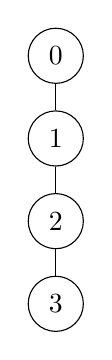
\begin{tikzpicture}[scale=0.7]
      \node [arn_x] {0}
        child {node [arn_x] {1}
          child {node [arn_x] {2}
            child {node [arn_x] {3}}}};
    \end{tikzpicture}
    \caption{Árvore linear.}
    \label{fig:arvorelinear}
\end{subfigure}
\hfill
  \begin{subfigure}[b]{0.3\textwidth}
      \centering
      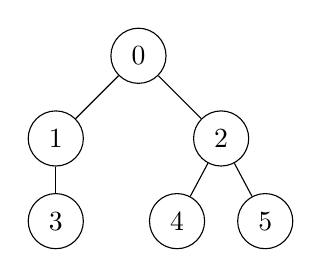
\begin{tikzpicture}[scale=0.7,
        level distance=1.5cm,
        level 1/.style={sibling distance=3cm},
        level 2/.style={sibling distance=1.6cm}]
        \node [arn_x] {0}
          child {node [arn_x] {1}
            child {node [arn_x] {3}}
          }
          child {node [arn_x] {2}
            child {node [arn_x] {4}}
            child {node [arn_x] {5}}
          };
      \end{tikzpicture}
      \caption{Árvore binária.}
      \label{fig:arvorebinaria}
  \end{subfigure}
  \hfill
  \begin{subfigure}[b]{0.3\textwidth}
      \centering
      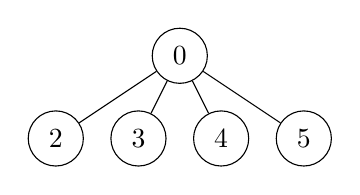
\begin{tikzpicture}[scale=0.7,
        level distance=1.5cm,
        level 1/.style={sibling distance=1.5cm}]
        \node [arn_x] {0}
          child {node [arn_x] {2}}
          child {node [arn_x] {3}}
          child {node [arn_x] {4}}
          child {node [arn_x] {5}};
      \end{tikzpicture}
      \caption{Árvore quaternária.}
      \label{fig:arvorequaternaria}
  \end{subfigure}
     \caption{Exemplos de árvores com fatores de ramificação diferentes.}
     \label{fig:ramificação}
\end{figure}

\subsection{Árvores completas}
Uma \textbf{árvore completa} é uma em que todos os níveis exceto possivelmente o último
estão completos, ou seja, todas as folhas se encontram no último nível e caso este não
esteja completo todos os nós devem estar o mais à esquerda possível.

\tikzset{
  treenode/.style = {align=center, minimum size=7mm, inner sep=0pt, text centered},
  arn_x/.style = {treenode, circle, draw=black, minimum size=7mm}
}
\begin{figure}[H]
  \centering
  \subcaptionbox{Nós não estão o mais à esquerda possível.}%
    [.4\linewidth]
    {
      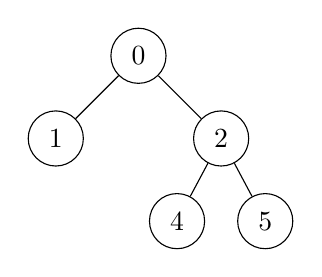
\begin{tikzpicture}[scale=0.7,
        level distance=1.5cm,
        level 1/.style={sibling distance=3cm},
        level 2/.style={sibling distance=1.6cm}]
        \node [arn_x] {0}
          child {node [arn_x] {1}}
          child {node [arn_x] {2}
            child {node [arn_x] {4}}
            child {node [arn_x] {5}}
          };
      \end{tikzpicture}
    }
  \hspace{1.2cm}
  \subcaptionbox{O terceiro nível não está completo (o nó 1 tem apenas um filho).}
    [.4\linewidth]{
      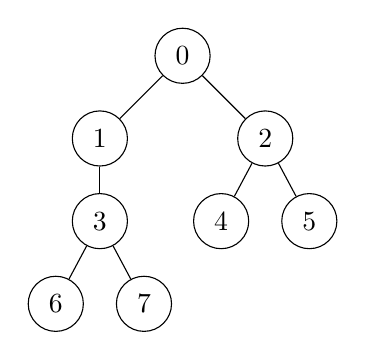
\begin{tikzpicture}[scale=0.7,
        level distance=1.5cm,
        level 1/.style={sibling distance=3cm},
        level 2/.style={sibling distance=1.6cm}]
        \node [arn_x] {0}
          child {node [arn_x] {1}
            child {node [arn_x] {3}
              child {node [arn_x] {6}}
              child {node [arn_x] {7}}
            }
          }
          child {node [arn_x] {2}
            child {node [arn_x] {4}}
            child {node [arn_x] {5}}
          };
      \end{tikzpicture}
    }
    \\
    \vspace{1.2cm}
  \subcaptionbox{Árvore binária completa.}
    [.4\linewidth]{
      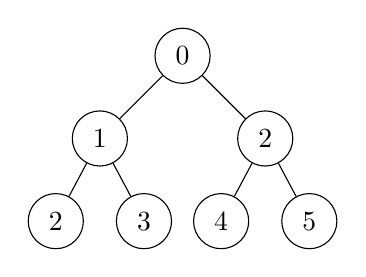
\begin{tikzpicture}[scale=0.7,
        level distance=1.5cm,
        level 1/.style={sibling distance=3cm},
        level 2/.style={sibling distance=1.6cm}]
        \node [arn_x] {0}
          child {node [arn_x] {1}
            child {node [arn_x] {2}}
            child {node [arn_x] {3}}
          }
          child {node [arn_x] {2}
            child {node [arn_x] {4}}
            child {node [arn_x] {5}}
          };
      \end{tikzpicture}
    }
  \hspace{1.2cm}
  \subcaptionbox{Árvore binária completa.}
    [.4\linewidth]{
      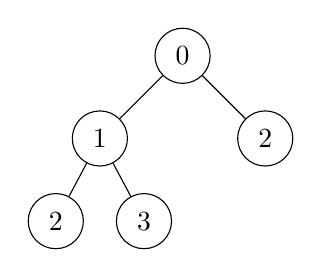
\begin{tikzpicture}[scale=0.7,
        level distance=1.5cm,
        level 1/.style={sibling distance=3cm},
        level 2/.style={sibling distance=1.6cm}]
        \node [arn_x] {0}
          child {node [arn_x] {1}
            child {node [arn_x] {2}}
            child {node [arn_x] {3}}
          }
          child {node [arn_x] {2}
          };
      \end{tikzpicture}
    }
    \caption{Exemplos de árvores completas ou não.}
  \end{figure}


\subsection{Busca em profundidade e travessias}
Árvores podem ser percorridas de diferentes maneiras partindo de sua raiz, podendo
``conhecer'' seus nós em ordens diferentes a depender de algum critério definido para
escolher o próximo nó a ser examinado. Em particular duas maneiras bastante conhecidas
para realizar a travessia de uma árvore são a \textbf{busca em profundidade} e a
\textbf{busca em largura}, onde a primeira tenta se aprofundar na árvore o máximo
possível antes de explorar outros caminhos e a segunda explora a árvore nível a nível,
conhecendo todos os nós de determinada profundidade antes de conhecer nós mais profundos.

Uma busca em profundidade também pode ser realizada de múltiplos jeitos, variando a ordem
em que o nó e seus filhos são processados. Uma \textbf{travessia em preordem} significa
que o nó será processado primeiro e então seus filhos serão colocados numa pilha de
execução da esquerda para a direita, enquanto numa \textbf{travessia em pós-ordem}
empilha os filhos do nó antes de processá-lo, como ilustrado na Figura
\ref{fig:travessias}.

\tikzset{
  treenode/.style = {align=center, minimum size=7mm, inner sep=0pt, text centered},
  arn_x/.style = {treenode, circle, draw=black, minimum size=7mm}
}

\begin{figure}[H]
  \centering
  \begin{subfigure}[b]{0.3\textwidth}
    \centering
    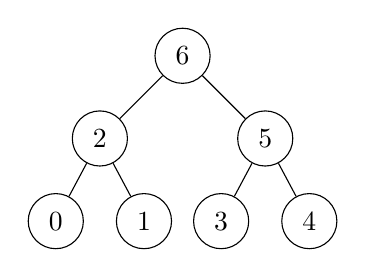
\begin{tikzpicture}[scale=0.7,
      level distance=1.5cm,
      level 1/.style={sibling distance=3cm},
      level 2/.style={sibling distance=1.6cm}]
      \node [arn_x] {6}
        child {node [arn_x] {2}
          child {node [arn_x] {0}
          }
          child {node [arn_x] {1}
          }
        }
        child {node [arn_x] {5}
          child {node [arn_x] {3}
          }
          child {node [arn_x] {4}
          }
        };
    \end{tikzpicture}
    \caption{Busca em profundidade em pós-ordem.}
    \label{fig:dfspost}
\end{subfigure}
\hfill
  \begin{subfigure}[b]{0.3\textwidth}
      \centering
      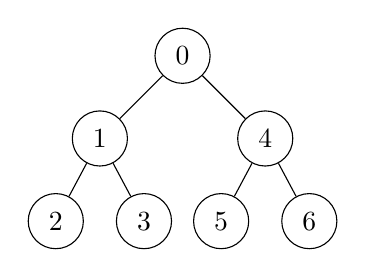
\begin{tikzpicture}[scale=0.7,
        level distance=1.5cm,
        level 1/.style={sibling distance=3cm},
        level 2/.style={sibling distance=1.6cm}]
        \node [arn_x] {0}
          child {node [arn_x] {1}
            child {node [arn_x] {2}
            }
            child {node [arn_x] {3}
            }
          }
          child {node [arn_x] {4}
            child {node [arn_x] {5}
            }
            child {node [arn_x] {6}
            }
          };
      \end{tikzpicture}
      \caption{Busca em profundidade em preordem.}
      \label{fig:dfspre}
  \end{subfigure}
  \hfill
  \begin{subfigure}[b]{0.3\textwidth}
      \centering
      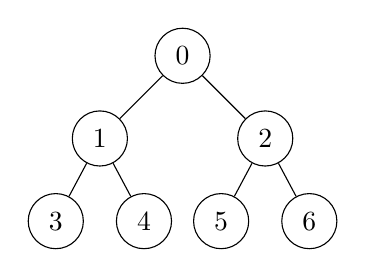
\begin{tikzpicture}[scale=0.7,
        level distance=1.5cm,
        level 1/.style={sibling distance=3cm},
        level 2/.style={sibling distance=1.6cm}]
        \node [arn_x] {0}
          child {node [arn_x] {1}
            child {node [arn_x] {3}
            }
            child {node [arn_x] {4}
            }
          }
          child {node [arn_x] {2}
            child {node [arn_x] {5}
            }
            child {node [arn_x] {6}
            }
          };
      \end{tikzpicture}
      \caption{Busca em largura.}
      \label{fig:bfs}
  \end{subfigure}
     \caption[Ordem de visita aos nós da árvore durante as travessias.]
      {\textbf{Ordem de visita aos nós da árvore durante as travessias.} O número do nó representa a ordem em que ele
      foi processado.}
     \label{fig:travessias}
\end{figure}

Para o escopo desta monografia é particularmente interessante a travessia em
\textbf{preordem}, que traz consigo algumas propriedades úteis a serem exploradas
mais a frente no texto, quando a implementação dos algoritmos for discutida. 